% =====================================================================
% Parte inicial do fonte RISTI / ICITS'27 (versão em português, revisão
% duplo-cega: sem autoria): título, resumo e palavras-chave em português e
% em inglês, dentro dos limites da RISTI (150 palavras, 5 palavras-chave).
% O corpo do artigo vem de paper_pt.tex. Use sync_risti.py para gerar
% paper_pt_risti.tex e paper_pt_risti_15p.tex, e build_risti_docx.py para
% gerar o .docx. Não é compilável com LaTeX.
% =====================================================================

\title{Uma Análise por Fluxo de Acesso em Redes Viárias Dirigidas: um Estudo em Grafos de Três Bairros do Rio de Janeiro}

\abstractpt{Modelamos as redes viárias de Urca, Copacabana e Botafogo como grafos
dirigidos do OpenStreetMap. Perguntamos se indicadores estruturais ou um
fluxo de acesso identificam um bairro com uma única rota de saída, e se
isso reflete a geografia ou o tamanho. Pontes e articulações fortes e o
corte mínimo entre dois nós não ordenam os bairros. O fluxo máximo do
núcleo do bairro até as portas administrativas ordena: uma rota disjunta por ruas
na Urca, dezoito em Copacabana e quinze em Botafogo, estável sob
variações de recorte e margem. Contar interseções em vez de ruas quase
não muda os valores, e respeitar o sentido das vias reduz o acesso das
malhas abertas a menos da metade, sem alterar a Urca. Pedaços das malhas
abertas do tamanho da Urca não reproduzem o padrão, associado à geografia
da península. A contagem pode ajudar a sinalizar bairros com uma só saída.}

\keywordspt{Fluxo máximo; Mobilidade urbana; Grafos dirigidos; Conectividade forte; Redes viárias}

\entitle{An Access-Flow Analysis of Directed Street Networks: A Graph Study of Three Rio de Janeiro Neighbourhoods}

\abstracten{We model the street networks of Urca, Copacabana and Botafogo as directed
graphs built from OpenStreetMap. We ask whether structural indicators or
an access flow identify a neighbourhood with a single exit route, and
whether this reflects geography or size. Strong bridges, strong
articulation points and the node-to-node minimum cut do not order the
neighbourhoods. The maximum flow from each core to its administrative
gateways does: one street-disjoint route for Urca, eighteen for
Copacabana and fifteen for Botafogo, stable under clip and margin
variations. Counting intersections instead of streets barely changes the
values, and respecting one-way directions cuts the open grids' access to
less than half without changing Urca. Pieces of the open grids the size of
Urca do not reproduce the pattern, which is tied to the peninsula's
geography. The count can help flag neighbourhoods with a single exit.}

\keywordsen{Maximum flow; Urban mobility; Directed graphs; Strong connectivity; Street networks}

% =====================================================================

\section{Introdução}
\label{sec:intro}

Redes viárias são comumente modeladas como grafos, cujos vértices são
interseções e cujas arestas são trechos de rua~\cite{boeing}. A direção
importa nesses grafos: sob regulamentação de mão única, uma interseção
pode ser alcançável sem oferecer caminho de volta. Saber por quantas rotas independentes um bairro
se liga ao restante da cidade interessa ao planejamento diante de uma
enchente, de um deslizamento ou da interdição de um túnel.

Métodos de conectividade localizam pontos críticos em redes viárias por
meio de pontes e pontos de articulação~\cite{tarjan1972depth}, estendidos
a grafos dirigidos~\cite{italiano2012finding}, e medidas de centralidade
o fazem por meio de escores por vértice~\cite{alatristasalas2019,kirkley2018betweenness}.
Essas medidas não contam as rotas independentes que ligam um bairro ao
exterior, e poucos estudos as contrastam entre bairros de geografia
distinta. Não está claro, então, se elas, ou uma medida de fluxo,
identificam um bairro que se alcança por uma única rota.

Comparamos a Urca, uma península cujas duas malhas residenciais se ligam
por um corredor (Figura~\ref{fig:networks}), com duas grandes malhas
abertas de orla, Copacabana e Botafogo. Aplicamos dois tipos de medida:
os indicadores estruturais dirigidos (pontes e articulações fortes) e o
fluxo de acesso, que é o fluxo máximo~\cite{edmonds1972theoretical} do
núcleo de cada bairro até suas portas de acesso, os pontos em que uma rua
cruza a fronteira. Pelo teorema do fluxo máximo e corte mínimo~\cite{ford1956maximal}, esse
fluxo é o menor número de ruas cujo fechamento isola o núcleo do bairro; contamos
também as interseções que precisam falhar, com e sem o sentido das vias.
A Urca é também a menor das três redes, e por
isso controlamos o tamanho com pedaços das malhas abertas e com modelos
nulos pareados por tamanho. Copacabana entra porque os dados do
OpenStreetMap trazem dois túneis rodoviários, Velho e Novo, em sua saída,
o que permite testar o quanto seu acesso depende deles.

O objetivo deste estudo exploratório é testar, em três bairros
contrastantes, se os indicadores estruturais dirigidos ou o fluxo de
acesso identificam um bairro de rota de acesso única, e se o resultado se
deve à geografia ou ao tamanho. O artigo contribui, ainda, com um
\emph{pipeline} reprodutível que constrói grafos viários dirigidos e
ponderados a partir do OpenStreetMap, recortados pelo polígono
administrativo oficial, com os algoritmos verificados contra o
\texttt{networkx}. A Seção~\ref{sec:related} revisa a literatura, a
Seção~\ref{sec:method} descreve o método, a Seção~\ref{sec:results} traz
os resultados, e as Seções~\ref{sec:discussion} e~\ref{sec:conclusion}
trazem a discussão e a conclusão.

% =====================================================================
\section{Trabalhos Relacionados}
\label{sec:related}

Pontes e pontos de articulação, cuja remoção desconecta um grafo, são
encontrados em tempo linear pela busca em profundidade~\cite{tarjan1972depth}.
Eles ignoram a direção. Italiano et al.~\cite{italiano2012finding} os
generalizaram para grafos dirigidos como pontes \emph{fortes} e pontos de
articulação \emph{fortes}, cuja remoção aumenta o número de componentes
fortemente conexas, e propuseram algoritmos de tempo linear. Essas
noções descrevem o grafo como um todo e não se referem a uma origem ou a
um destino.

A centralidade de intermediação identifica interseções e trechos de rua
críticos em cidades densamente povoadas~\cite{alatristasalas2019}, e
Kirkley et al.~\cite{kirkley2018betweenness} a estudam em redes viárias.
A sintaxe espacial calcula integração e escolha sobre o mapa axial ou de
segmentos de um assentamento~\cite{hillier1984social}. Essas abordagens
ordenam vértices ou segmentos e não contam as rotas independentes que
ligam uma região ao exterior.

Outros estudos tratam da direção das vias e da redundância de rotas. Yu e
Gayah~\cite{yu2020resilience} comparam três configurações de rede viária,
entre elas a de mão única, sob falhas de trechos e encontram uma troca
entre eficiência e resiliência nas redes com restrições de movimento.
El-Rashidy e Grant-Muller~\cite{elrashidy2016redundancy} propõem índices
de redundância de cruzamentos e da rede que incluem o número de rotas
alternativas. Esses trabalhos avaliam a redundância de interseções ou da
rede inteira, sem tratar o acesso de um bairro ao restante da cidade.

Estudos de resiliência medem como o serviço se degrada sob falha. Rouhana
e Jawad~\cite{rouhana2020} avaliam com SIG o papel da topologia da rede,
Alatrista-Salas et al. simulam falhas aleatórias e direcionadas, Ientile
et al.~\cite{ientile2022measuring} propõem um índice de perda de
capacidade de serviço, e Ganin et al.~\cite{ganin2017resilience} comparam
eficiência e resiliência em 40 áreas urbanas dos EUA. Em geral, esses
estudos tomam a rede inteira como unidade de análise, sem isolar o acesso
de uma região específica.

Fluxo máximo e corte mínimo, ligados pelo teorema de Ford e
Fulkerson~\cite{ford1956maximal}, são os instrumentos mais próximos dos
que usamos e têm sido aplicados a redes viárias para estudar isolamento e
falha geográfica. Sugiura e Kurauchi~\cite{sugiura2023isolation} definem
um índice de vulnerabilidade de isolamento como a solução de um problema
de fluxo máximo entre bases de apoio e de recepção e propõem um método
para encontrar todos os conjuntos de elos que geram isolamento. Otsuki et
al.~\cite{otsuki2016improved} propõem algoritmos mais rápidos de fluxo
máximo e corte mínimo sob falhas geográficas modeladas como discos
circulares e os aplicam a uma rede viária de Nova York. Seguimos essa
dualidade, com a região de origem e o sumidouro definidos pelo próprio
bairro: seu núcleo e as ruas que cruzam sua fronteira oficial. Nos
trabalhos revistos, não encontramos a contagem de rotas disjuntas entre o
núcleo de um bairro e suas portas administrativas, nem a comparação
dessa contagem entre bairros de geografia distinta com controle de
tamanho.

% =====================================================================
\section{Metodologia}
\label{sec:method}

\subsection{Dados e construção do grafo}
\label{sec:data}

Para cada bairro, consultamos a API Overpass do OpenStreetMap em busca
das vias trafegáveis (classes de \texttt{highway} de \emph{motorway} a
\emph{residential}, \emph{living\_street}, \emph{road} e as variantes
\texttt{*\_link}; vias de serviço, trilhas e vias de pedestre ficam de
fora) dentro de um envelope de busca, e armazenamos em cache a resposta.
Os extratos datam de 21 de setembro de 2026 (Copacabana) e de 23 de
setembro de 2026 (Urca e Botafogo). Os dados do mapa são
\textcopyright{} colaboradores do OpenStreetMap (ODbL).

Cada trecho de rua torna-se um arco dirigido que respeita sua
\emph{tag} \texttt{oneway}; rotatórias, \emph{motorways} e
\emph{trunk links} são de mão única por convenção do OpenStreetMap, e os
demais trechos são de mão dupla. Pontos de forma de grau dois são
contraídos, como no OSMnx~\cite{boeing}, de modo que os vértices sejam
interseções verdadeiras; sem essa etapa, cada curva de uma rua seria um
falso ponto de articulação. Cadeias que retornam ao próprio vértice ou
cujos trechos não compartilham um sentido são descartadas (0,25\% a
0,8\% das cadeias), e ruas paralelas entre o mesmo par de interseções
são mantidas (3, 2 e 4 pares). As coordenadas são projetadas em metros, e
cada aresta é ponderada por seu tempo de percurso, a soma dos
comprimentos de seus trechos sobre a velocidade. A velocidade é a
\emph{tag} \texttt{maxspeed} quando existe, e um padrão por classe de
via caso contrário (ver o README); apenas 34\%, 32\% e 18\% das vias na
Urca, em Copacabana e em Botafogo trazem \texttt{maxspeed}.


A extensão de um bairro é uma escolha de modelagem. Tomamos o polígono
oficial (Instituto Pereira Passos / Data.Rio~\cite{ipp_bairros},
acessado em setembro de 2026) como a fronteira nos três casos. Um
retângulo delimitador traçado manualmente serve apenas como envelope de
busca, unido ao retângulo delimitador do próprio polígono, e o grafo é
recortado pelo polígono antes de qualquer análise, de modo que nenhuma
diferença entre os bairros decorra de um pré-processamento desigual.
Ruas que cruzam a fronteira são cortadas ali e servem apenas para
identificar as portas de acesso (Seção~\ref{sec:access-flow}). A
Seção~\ref{sec:res-clip} compara o resultado com o retângulo manual
isolado. A Tabela~\ref{tab:redes} e a Figura~\ref{fig:networks} descrevem as
redes resultantes: de 75\% a 91\% dos trechos de rua são de mão única, e
de 4\% a 10\% das interseções ficam fora do núcleo fortemente conexo (ou
núcleo forte), a maior componente fortemente conexa (CFC) do grafo
dirigido, em que toda interseção alcança todas as outras.

\begin{table}[t]
\centering
\caption{Redes após a simplificação topológica (OpenStreetMap), as três
recortadas pelo polígono administrativo oficial do bairro.}
\label{tab:redes}
\begin{tabular}{lrrr}
\toprule
 & Urca & Copacabana & Botafogo \\
\midrule
Interseções ($V$)                     & 70   & 345  & 434 \\
Trechos de rua                        & 104  & 494  & 563 \\
Trechos de mão única (\%)             & 91,3 & 74,9 & 76,2 \\
Núcleo fortemente conexo ($V$)        & 65   & 331  & 392 \\
Fora do núcleo forte (\% de $V$)    & 7,1  & 4,1  & 9,7 \\
\bottomrule
\end{tabular}
\end{table}

\begin{figure}[t]
\centering
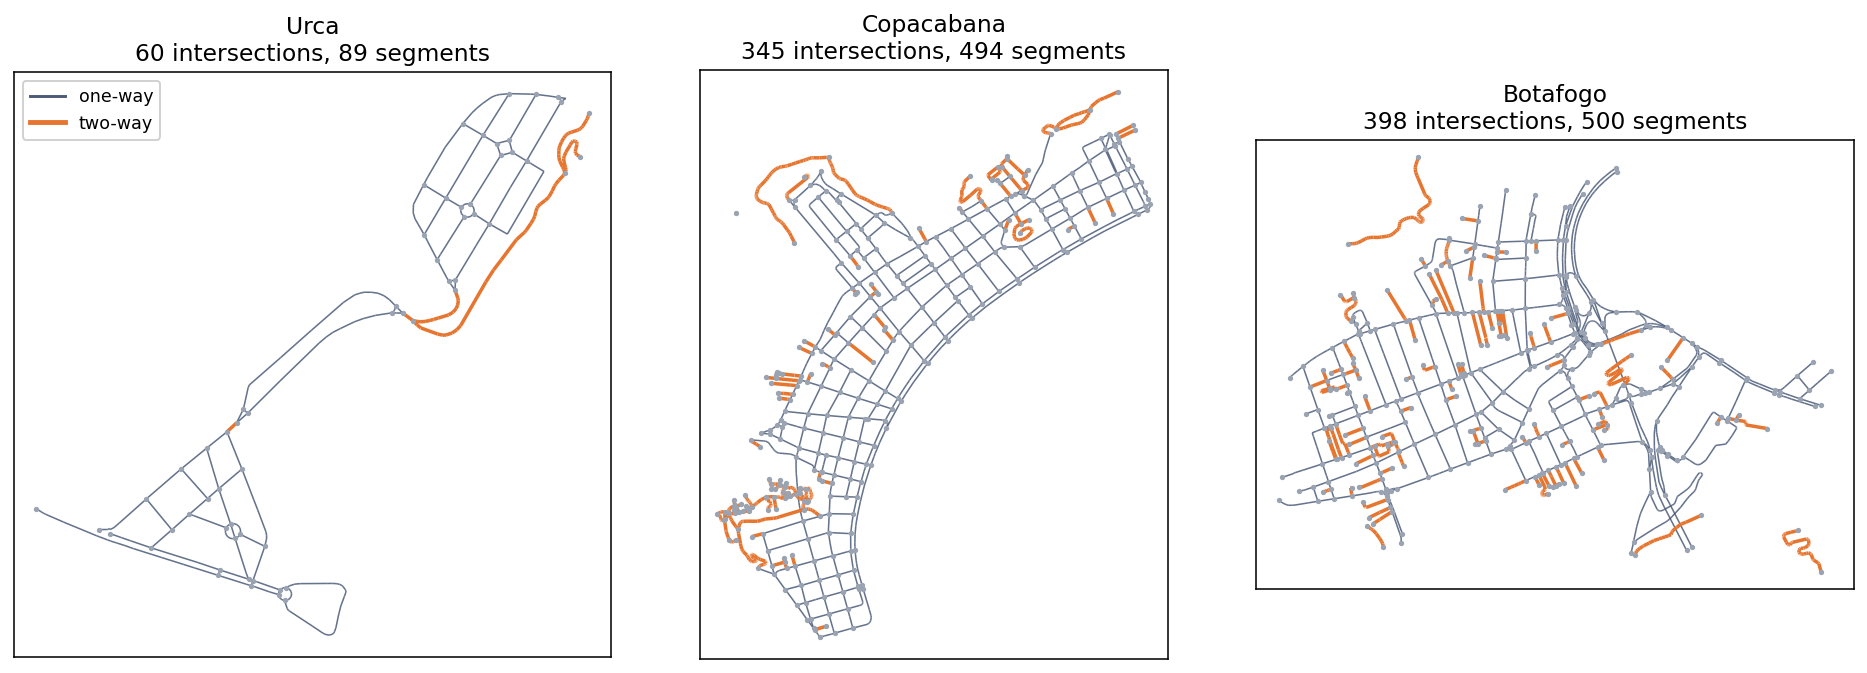
\includegraphics[width=\textwidth]{Figures/fig_networks.png}
\caption{As três redes dos bairros após a simplificação topológica e o
recorte pelo polígono oficial (mão única em escuro, mão dupla em
laranja). A Urca é uma península cujas duas malhas se encontram em um
único corredor; Copacabana e Botafogo são grandes malhas abertas.}
\label{fig:networks}
\end{figure}

\subsection{Indicadores estruturais e algoritmos}
\label{sec:algos}

Calculamos quatro indicadores estruturais, cada um como uma proporção
(Tabela~\ref{tab:estrutural}). Pontes fracas são ruas cuja remoção
desconecta o grafo não dirigido, e são reportadas como percentual de
todos os trechos de rua. Pontes fortes são ruas cujo fechamento faz o
núcleo forte deixar de ser fortemente conexo, e pontos de articulação fortes
são interseções cuja remoção faz o mesmo~\cite{italiano2012finding};
são reportados como percentual das ruas e das interseções do núcleo forte,
respectivamente. O quarto indicador é a percentagem de interseções fora
do núcleo forte. Nos indicadores estruturais, fechar uma rua remove os dois
sentidos e todos os trechos paralelos entre suas duas interseções, e
ruas paralelas nunca são pontes fracas. Nos cálculos de fluxo, cada rua
paralela tem capacidade unitária.

Todas as análises usam um grafo dirigido e ponderado, representado por
lista de adjacência. As componentes são encontradas por busca em
largura, as CFC pela interseção da alcançabilidade direta com a reversa,
e as pontes e articulações fracas, diretamente a partir de sua
definição. Pontes e articulações fortes são encontradas recalculando as
CFC após cada remoção, e não com o algoritmo de tempo linear de Italiano
et al.~\cite{italiano2012finding}; isso levou 0,1\,s, 4,2\,s e 10,2\,s para Urca, Copacabana e
Botafogo. O fluxo máximo e o corte mínimo, o menor conjunto de ruas cujo
fechamento separa a origem do destino, usam
Edmonds--Karp~\cite{edmonds1972theoretical} com capacidade unitária por
rua em ambos os sentidos, de modo que o fluxo seja igual ao número de
rotas disjuntas por ruas. A intermediação segue Brandes~\cite{brandes2001faster}, com o algoritmo
de Dijkstra~\cite{dijkstra1959note} para os pesos de tempo de percurso.
A intermediação de uma interseção é a fração dos pares ordenados do
núcleo fortemente conexo cujo caminho de tempo mínimo passa por ela; o
cálculo divide empates, exclui os extremos e normaliza por $(n-1)(n-2)$.

Conferimos as implementações contra o \texttt{networkx} nas três redes
(\texttt{test\_vs\_networkx.py}, \texttt{test\_betweenness.py}).
Componentes, CFC, pontes e articulações fracas, caminhos mínimos, fluxo
máximo e intermediação conferem. Pontes e articulações fortes, que o
\texttt{networkx} não calcula, conferem com uma recontagem independente
das CFC após cada remoção.

\subsection{Fluxo de acesso por portas}
\label{sec:access-flow}

Para medir o acesso ao restante da cidade, em vez da separação entre
duas interseções escolhidas, distinguimos o \emph{interior} de um bairro
de suas \emph{portas de acesso}. A rede viária também é extraída com uma
margem de 400\,m além do polígono oficial, de modo que a primeira
interseção além da fronteira esteja presente em toda rua que a cruze.
Um vértice da rede recortada é uma \emph{porta de acesso} se ao menos
uma de suas ruas incidentes cruza a fronteira; todo outro vértice é
\emph{interior}. Como uma porta de acesso pode admitir tráfego em apenas
um sentido, restringimos os dois conjuntos ao maior componente
\emph{não dirigido}, e não ao núcleo fortemente conexo: uma saída de mão
única ainda é uma saída real.

A região de origem é formada pelas $k=\mathrm{round}(f\,n)$ interseções
interiores mais distantes, em número de arestas, da porta de acesso mais
próxima, com $n$ o tamanho desse componente e $f=0{,}2$; ela é o núcleo
do bairro. Uma superfonte alimenta a região de origem, e o conjunto de
portas de acesso alimenta um superssumidouro, ambos com capacidade
infinita, e o Edmonds--Karp é executado entre eles. O valor resultante,
o \emph{fluxo de acesso}, é o número de rotas disjuntas por ruas entre o
núcleo do bairro e as saídas para o restante da cidade.

Com a mesma origem e as mesmas portas, calculamos duas variantes e sua
combinação. A primeira conta rotas disjuntas por \emph{interseções}
(teorema de Menger~\cite{menger1927}): dividindo cada vértice em $v_{\text{ent}}\to
v_{\text{sai}}$, só as interseções interiores recebem capacidade~1,
enquanto o núcleo do bairro e as portas ficam incortáveis (capacidade
infinita) e as ruas têm capacidade infinita; sem essa distinção, o valor
ficaria limitado trivialmente pelo número de portas. A segunda respeita o
\emph{sentido} das vias, atribuindo capacidade unitária por arco, e não
nos dois sentidos de cada rua: uma saída de mão única só conta no sentido
que de fato permite deixar o bairro, de modo que o fluxo de acesso
dirigido é menor ou igual ao não dirigido. A combinação divide os
vértices e mantém apenas os arcos que existem, e conta as interseções
que precisam falhar quando o sentido das vias é respeitado.
As duas contagens correspondem a eventos diferentes: o fechamento de
ruas, como numa interdição ou num deslizamento, e a falha de
interseções, como num alagamento ou no bloqueio de um cruzamento. Em
ambos os casos, o valor do fluxo é o menor número de falhas que isolam
o núcleo do bairro de todas as portas. As quatro contagens de rotas (por ruas e por interseções, sem e
com o sentido das vias) conferem com o \texttt{networkx}
(\texttt{ruas\_vs\_intersecoes.py}).

\subsection{Controles e análises de sensibilidade}
\label{sec:controls}

\emph{Corte mínimo entre dois nós.} Como referência, calculamos o corte
mínimo entre 300 pares aleatórios de interseções no maior componente não
dirigido de cada rede.

\emph{Localização do corte de acesso.} Um corte mínimo não é único, e o
que o Edmonds--Karp devolve é o mais próximo da origem. Por isso,
também enumeramos toda rua cujo fechamento sozinho separa a região de
origem de todas as portas, contamos as interseções de cada lado, e
conferimos se suas interseções extremas coincidem com as cinco mais
centrais por intermediação. Repetimos isso para $f$ de 0,05 a 0,5.

\emph{Controle de tamanho do fluxo de acesso.} Sorteamos pedaços conexos
de 70 interseções, o tamanho da Urca, dentro de Copacabana e de Botafogo,
tratamos cada um como um bairro e calculamos seu fluxo de acesso; as
portas de um pedaço são suas interseções ligadas por uma rua a uma
interseção fora dele. Sorteamos 500 pedaços por bairro por crescimento em
busca em largura e 500 por crescimento aleatório (modelo de Eden), e
acrescentamos uma busca de subida de encosta que troca uma interseção por
vez para minimizar o fluxo (8 reinícios de 1.500 iterações).

\emph{Controle de tamanho da intermediação.} Sorteamos 300 pedaços
conexos de 65 a 78 interseções por bairro e por modo de crescimento,
mantemos os cujo núcleo fortemente conexo tem de 60 a 70 vértices (o da
Urca tem 65), e comparamos o máximo da Urca com o deles. Também
calculamos o produto do máximo por $\sqrt{n}$ e religamos as arestas de cada núcleo forte preservando os graus (50 religações por rede, não dirigida e
sem peso). Em cada nulo, o escore $z$ é a diferença entre o valor
observado e a média do nulo, dividida pelo desvio padrão do nulo. A
religação destrói a planaridade, e por isso qualquer rede viária real
aparece como extrema diante desse nulo; o nulo informativo é o pareado
por tamanho, e a religação serve como verificação.

\emph{Extensão, fração de origem, margem e túneis.} Repetimos a análise
com o retângulo manual, sem recorte e com as portas de acesso na borda
do retângulo, e variamos $f$ (0,15, 0,20, 0,25) e a margem (200, 400 e
800\,m). Uma porta é uma saída de túnel quando a rua que sai por ela
passa a até 2\,m de um nó de uma via marcada \texttt{tunnel=yes} ou
\texttt{building\_passage}; recalculamos o fluxo sem essas portas. Todos
os procedimentos aleatórios usam sementes fixas, e o README do
repositório (omitido para a revisão) lista o script de cada tabela e
figura.

% =====================================================================
\section{Resultados}
\label{sec:results}

\subsection{Os indicadores estruturais não ordenam os casos}
\label{sec:res-struct}

A Tabela~\ref{tab:estrutural} compara os indicadores estruturais
dirigidos. A Urca não ocupa o mesmo extremo em todos eles. Tem o maior
valor de articulações fortes (73,8\%, contra 54,1\% em Copacabana e
63,5\% em Botafogo) e o menor de pontes fracas (10,6\%, contra 15,8\% e
20,2\%), com valores intermediários em pontes fortes (61,5\%) e na
fração fora do núcleo forte (7,1\%). Por isso os indicadores não
ordenam os bairros de forma consistente.

As duas malhas abertas também diferem entre si. Em pontes fortes,
Copacabana tem 45,3\% e Botafogo 68,4\%, e a diferença persiste quando
as redes são construídas a partir do retângulo manual
(Seção~\ref{sec:res-clip}). Em todos os bairros, de 45\% a 68\% das
ruas do núcleo forte são pontes fortes; na Urca, são 59 das 96.

\begin{table}[t]
\centering
\caption{Indicadores estruturais dirigidos (normalizados), com as três
redes recortadas pelo polígono oficial.}
\label{tab:estrutural}
\begin{tabular}{lrrr}
\toprule
 & Urca & Copacabana & Botafogo \\
\midrule
Pontes fracas (\% dos trechos)          & 10,6 & 15,8 & 20,2 \\
Pontes fortes (\% das ruas do núcleo forte)   & 61,5 & 45,3 & 68,4 \\
Articulações fortes (\% do núcleo forte)      & 73,8 & 54,1 & 63,5 \\
Fora do núcleo forte (\% de $V$)        & 7,1  & 4,1  & 9,7 \\
\bottomrule
\end{tabular}
\end{table}

\subsection{Corte mínimo entre dois nós}
\label{sec:res-mincut}

Em 300 pares aleatórios de interseções por bairro
(Seção~\ref{sec:controls}), o corte mínimo, em número de ruas, varia de
1 a 3 na Urca e em Botafogo e de 1 a 4 em Copacabana. Os pares com corte
1 são 70,0\% na Urca, 40,7\% em Copacabana e 52,0\% em Botafogo, e as
médias são 1,49, 1,98 e 1,69. A Urca tem os menores valores, e a
diferença entre sua média e a das malhas abertas é de 0,2 a 0,5 rua.

\subsection{Fluxo de acesso por portas}
\label{sec:res-access}

O fluxo de acesso, em rotas disjuntas por ruas, é 1 na Urca, 18 em
Copacabana e 15 em Botafogo (Tabela~\ref{tab:acesso}), com 3, 21 e 31
portas. Os valores não mudam para $f$ entre 0,15 e 0,25 nem para
margens de 200 a 800\,m. A Urca não tem portas de túnel. Em Copacabana,
quatro das 21 portas são saídas dos túneis Velho e Novo, e sem elas o
fluxo é 15. Em Botafogo, quatro das 31 portas também são saídas desses
túneis, e o fluxo permanece em 15. A Seção~\ref{sec:res-ruas-int} traz
as contagens por interseções e com o sentido das vias.

\begin{table}[t]
\centering
\caption{Fluxo de acesso por portas: rotas disjuntas do núcleo de cada
bairro até suas portas de acesso administrativas, contadas por ruas e
por interseções (teorema de Menger), sem e com o sentido das vias
($f=0{,}2$ e margem de 400\,m).}
\label{tab:acesso}
\begin{tabular}{lrrr}
\toprule
 & Urca & Copacabana & Botafogo \\
\midrule
Portas de acesso identificadas                       & 3 & 21 & 31 \\
Rotas disjuntas por ruas                             & 1 & 18 & 15 \\
Rotas disjuntas por interseções                      & 1 & 17 & 14 \\
Rotas por ruas, respeitando o sentido                & 1 & 8  & 7 \\
Rotas por interseções, respeitando o sentido         & 1 & 8  & 6 \\
\bottomrule
\end{tabular}
\end{table}

\subsection{Contagens por ruas e por interseções}
\label{sec:res-ruas-int}

Sem o sentido das vias, contar interseções em vez de ruas muda pouco os
valores: 1, 17 e 14, contra 1, 18 e 15 (Tabela~\ref{tab:acesso}). Na
Urca, o fechamento de uma única rua do corredor, ou a falha de uma única
interseção dele, deixa o núcleo do bairro sem saída (Figura~\ref{fig:cut}). Em
Copacabana e Botafogo, o corte mínimo tem 18 e 15 ruas, ou 17 e 14
interseções, espalhadas pelo bairro.

Com o sentido das vias respeitado, o fluxo de acesso é 1 na Urca, 8 em
Copacabana e 7 em Botafogo, menos da metade do valor não dirigido nas
duas malhas abertas. Por interseções, os valores são 1, 8 e 6. As duas
contagens dirigidas coincidem na Urca e em Copacabana e diferem em uma
unidade em Botafogo. A Urca fica em uma única rota nas quatro contagens.

\subsection{Localização do corte de acesso}
\label{sec:res-cut}

Na Urca há três cortes de uma única rua, todos no corredor que liga as
duas malhas residenciais (Figura~\ref{fig:cut}): uma rua de 165\,m no
extremo nordeste, que é o corte devolvido pelo Edmonds--Karp e deixa 23
interseções do lado da origem; uma rua de 32\,m adjacente a ela, com 27;
e uma rua de 33\,m na junção sudoeste, com 33. O corte por interseções é
uma única interseção do corredor. Os três cortes aparecem para todo $f$
de 0,05 a 0,25 e têm as mesmas cinco interseções nas extremidades. Para
$f$ maior, restam dois cortes em $f=0{,}3$, um em $f=0{,}4$ e nenhum em
$f=0{,}5$. Copacabana e Botafogo não têm corte de uma única rua: seus
cortes mínimos têm 18 e 15 ruas, espalhadas pelo bairro.

\begin{figure}[t]
\centering
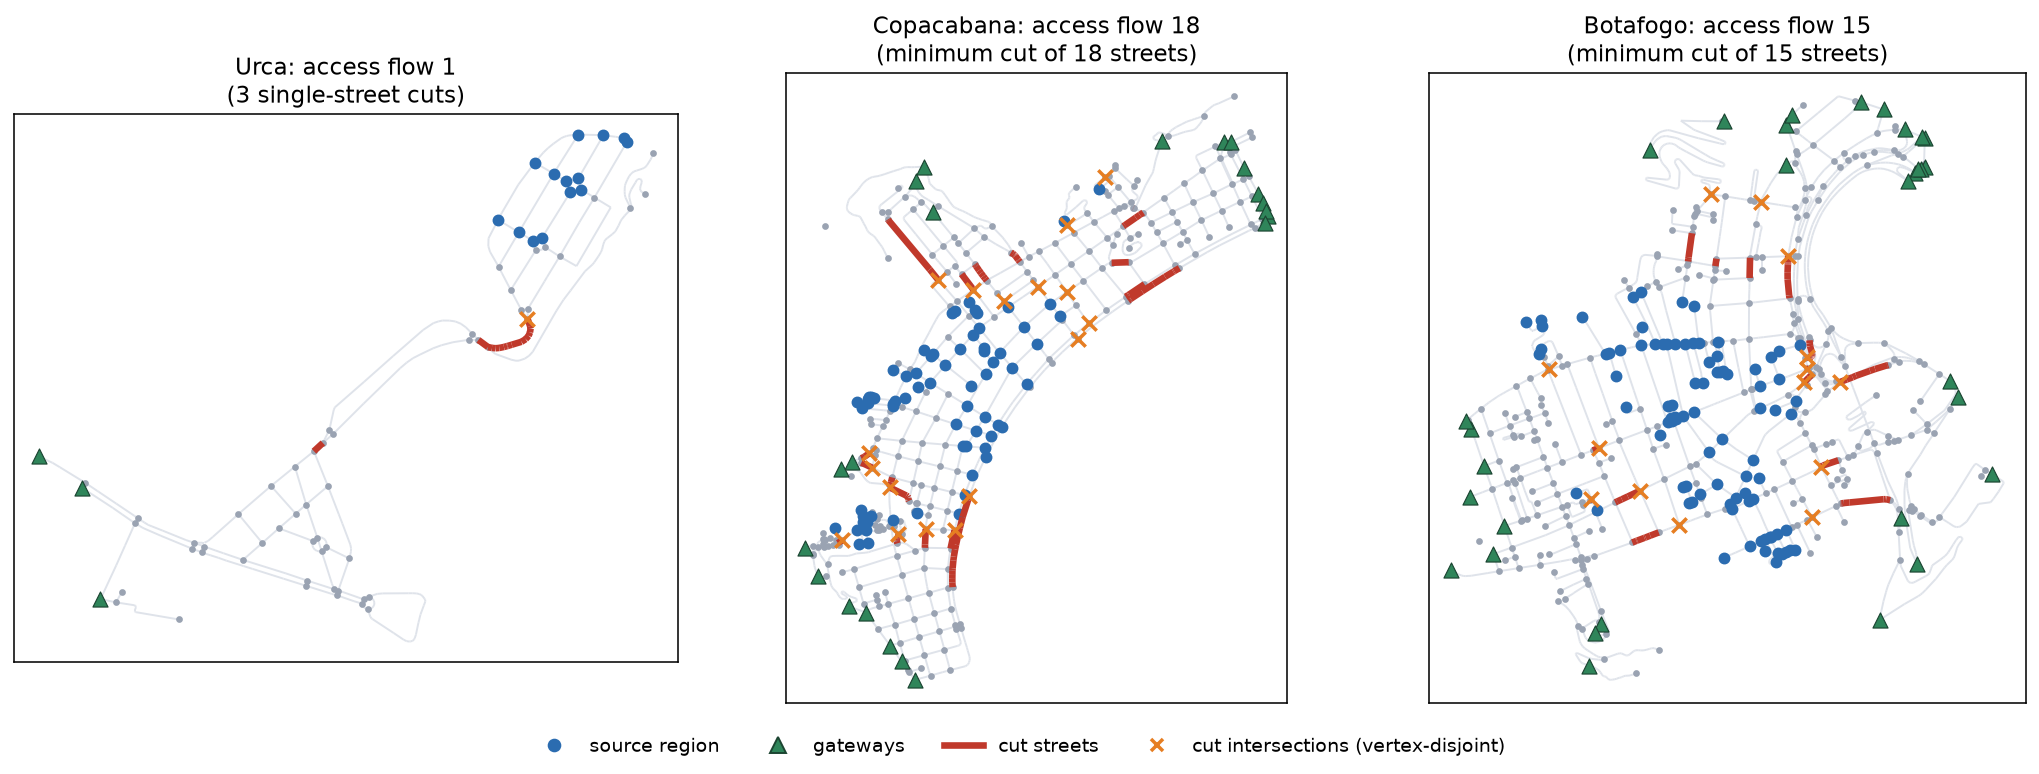
\includegraphics[width=\textwidth]{Figures/fig_cut.png}
\caption{Onde está o corte de acesso ($f=0{,}2$). Azul: região de
origem; verde: portas de acesso; vermelho: ruas de corte; laranja:
interseções de corte (contagem por vértices).}
\label{fig:cut}
\end{figure}

\subsection{Intermediação dirigida}
\label{sec:res-betweenness}

Na
Urca, as cinco interseções de maior intermediação ficam ao
longo do corredor e em suas junções com as duas malhas, com valores de
45,8\% a 54,2\%; elas são os extremos dos três cortes de uma única rua.
Em Copacabana e Botafogo, os máximos são 27,8\% e 22,4\%, ao longo do
eixo principal de Copacabana e de duas ruas paralelas em Botafogo.

O produto do máximo por $\sqrt{n}$, que seria constante se o máximo
escalasse como $n^{-1/2}$, é 4,4 na Urca, 5,1 em Copacabana e 4,4 em
Botafogo. Nos pedaços pareados por tamanho (Seção~\ref{sec:controls},
Figura~\ref{fig:controles}b), o máximo da Urca, 54,2\%, é igualado ou
superado por 2,0\% e 18,3\% dos pedaços de Copacabana e por 43,7\% e
51,8\% dos de Botafogo, nos modos de crescimento por busca em largura e
por Eden. Cada grupo tem 300 pedaços, exceto Botafogo por Eden, com 56.
Os escores $z$ da Urca vão de $-0{,}3$ a 1,9. A religação das arestas
preservando os graus dá escores $z$ de 22 a 39 nos três bairros.


\subsection{Controle de tamanho do fluxo de acesso}
\label{sec:res-controls}

A Urca é a menor das três redes. Para separar o efeito do tamanho,
comparamos seu fluxo de acesso com o de pedaços conexos de 70
interseções, o tamanho da Urca, sorteados dentro de Copacabana e de
Botafogo (Seção~\ref{sec:controls}). Nenhum dos 2.000 pedaços chegou a um
fluxo de 1 (Figura~\ref{fig:controles}a). A mediana do fluxo foi 11 e 13
nos pedaços de Copacabana e 8 e 11 nos de Botafogo, por crescimento em
busca em largura e por Eden, e todo pedaço teve ao menos 9 portas,
contra 3 na Urca. Os pedaços com fluxo de 3 ou menos foram 17,4\% e
10,8\% em Copacabana e 0,0\% e 0,2\% em Botafogo. A busca de subida de
encosta, que procura o menor fluxo possível, encontrou 3 como menor
valor, em pedaços com 53 portas em Copacabana e 45 em Botafogo.

\begin{figure}[t]
\centering
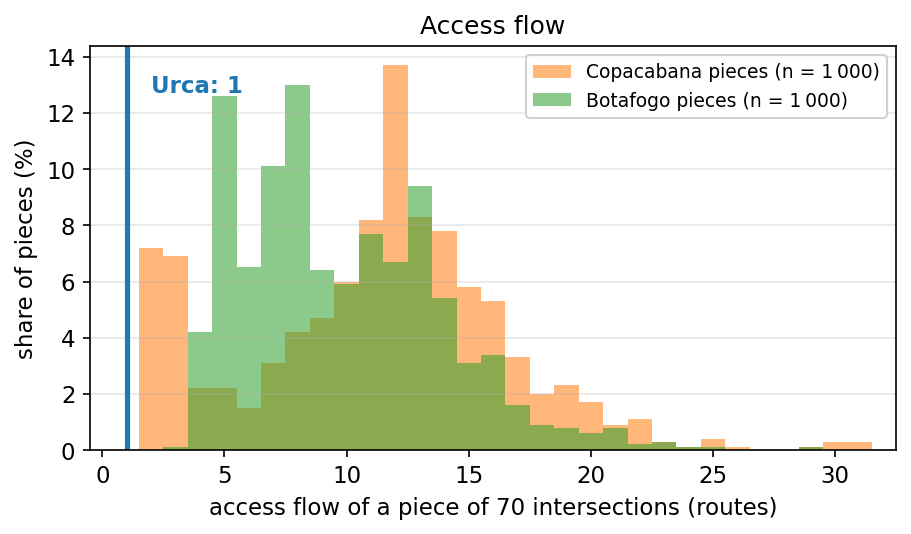
\includegraphics[width=\textwidth]{Figures/fig_controles.png}
\caption{Controles de tamanho. (a) Fluxo de acesso de pedaços conexos de
70 interseções sorteados dentro de Copacabana e Botafogo (500 por
crescimento em busca em largura e 500 por crescimento aleatório cada);
o fluxo da Urca é 1. (b) Máximo de intermediação dos pedaços pareados
por tamanho (Seção~\ref{sec:controls}); o da Urca é 54,2\%.}
\label{fig:controles}
\end{figure}

\subsection{Sensibilidade ao recorte}
\label{sec:res-clip}

Comparamos o polígono oficial com o retângulo
manual, sem recorte e com as portas na borda do retângulo. Do retângulo
para o polígono, os valores de Botafogo mudam pouco: as pontes fortes
vão de 70,4\% para 68,4\% e o fluxo de acesso de 16 para 15. Em
Copacabana, o retângulo incluía 158 de suas 496 interseções, que ficam no
território oficial de Botafogo, e as pontes fortes caem de 53,1\% para
45,3\% e as portas de 45 para 21. Na Urca, o retângulo truncava a
península, e o núcleo forte passa de 37 para 65 interseções e a fração
fora dele de 38,3\% para 7,1\%.

Duas comparações se repetem nos dois recortes. A diferença de pontes
fortes entre Copacabana e Botafogo é de 53,1\% contra 70,4\% com o
retângulo e de 45,3\% contra 68,4\% com o polígono. O fluxo de acesso da
Urca é 1, contra 13 a 18 em Copacabana e 15 a 16 em Botafogo. A fração
da Urca fora do núcleo forte e o número de portas, por sua vez, mudam
com o recorte.


% =====================================================================
\section{Discussão}
\label{sec:discussion}

Entre as medidas testadas, só o fluxo de acesso por portas isola a Urca
das duas malhas abertas. Ele separa a Urca nas redes não dirigida e
dirigida, e pedaços das malhas abertas com o tamanho da Urca não
reproduzem seu valor. Os indicadores estruturais dirigidos e o corte
mínimo entre dois nós não ordenam os bairros, e o máximo de intermediação
acompanha o tamanho do núcleo forte. O padrão de rota única associa-se, assim,
à geografia da península, nestes três casos.

Pontes e articulações fortes são calculadas sobre o núcleo fortemente
conexo e, nessas redes de mão única, de 45\% a 68\% das ruas do núcleo
forte são pontes fortes em qualquer bairro. Esses indicadores descrevem a
redundância interna do
núcleo forte, que é alta nos três bairros. O corte
mínimo entre dois nós mede quantas ruas separam dois pontos escolhidos, e
a resposta é pequena em toda parte. O fluxo de acesso toma o núcleo do bairro como
origem e as travessias da fronteira como sumidouro, e por isso mede a
ligação do bairro com o restante da cidade.

Na Urca, essa ligação passa por um corredor: três cortes de uma única rua
em série e, na contagem por interseções, uma única interseção
(Figura~\ref{fig:cut}). O bairro tem 0,21 porta por quilômetro de
perímetro do polígono oficial, contra 1,64 em Copacabana e 2,55 em
Botafogo, porque suas saídas se concentram em um único extremo e o
restante do perímetro é água e encosta. Um pedaço sorteado dentro de uma
malha tem, por construção, a fronteira cercada de malha e por isso muitas
portas. A intermediação localiza o corredor, pois seus maiores valores
ficam nos extremos dos três cortes, mas o valor máximo acompanha o
tamanho do núcleo forte. Os túneis de Copacabana não criam um gargalo
comparável: sem as quatro portas de túnel, o fluxo cai de 18 para 15.

Kirkley et al.~\cite{kirkley2018betweenness} mostram, em redes viárias de
97 cidades, que a distribuição estatística da intermediação é invariante
em redes planares e que a distribuição espacial dos vértices de maior
intermediação discrimina melhor entre cidades. Nossos dados seguem essa
direção: o máximo acompanha o tamanho do núcleo forte, e a posição dos vértices
de maior intermediação revela o corredor da Urca. Ganin et
al.~\cite{ganin2017resilience} encontram, em 40 áreas urbanas dos EUA,
que sistemas viários ineficientes podem ser resilientes e que alguns
eficientes são frágeis. O fluxo de acesso mede a redundância de saída,
que é distinta da eficiência do trânsito, e nossa comparação não testa
essa relação. Sugiura e Kurauchi~\cite{sugiura2023isolation} observam que
o conjunto de elos que define a vulnerabilidade de isolamento não precisa
ser único; na Urca, cada uma de três ruas em série isola sozinha
o núcleo do bairro.

Para o planejamento, a Urca é isolada por uma única falha, de rua ou de
interseção, e as malhas abertas exigem de 6 a 18, conforme o modelo de
falha. Um órgão de mobilidade ou de defesa civil trataria a Urca como um
ponto único a proteger ou a ter alternativa. Como poucas rotas de acesso
compartilham uma junção, as contagens por ruas e por interseções diferem
pouco, e a conclusão vale para os dois tipos de evento. Ignorar o sentido
das vias superestima a redundância das malhas abertas: de 18 rotas passa-se
a 8 em Copacabana, e de 15 a 7 em Botafogo.

O estudo tem três casos e não permite inferência estatística. A fronteira
administrativa define as portas, e um bairro nem sempre é uma unidade de
mobilidade; a extensão da rede é uma escolha de modelagem, como mostrou o
retângulo manual (Seção~\ref{sec:res-clip}). O fluxo usa capacidade
unitária por rua, sem considerar largura nem número de faixas, e conta
falhas necessárias na estrutura da rede, sem medir sua probabilidade nem o
volume de tráfego. Os tempos de percurso vêm, em sua maioria, de
velocidades padrão, e a conectividade depende da qualidade das
\emph{tags} \texttt{oneway}. Os pedaços de controle são recortes
arbitrários, e a busca por pedaços de fluxo mínimo dá um limite
heurístico.


% =====================================================================
\section{Conclusões}
\label{sec:conclusion}

Este estudo perguntou se indicadores estruturais dirigidos ou um fluxo de
acesso identificam um bairro com uma única rota de saída, e se isso
reflete a geografia. Em três bairros do Rio de Janeiro, só o fluxo de
acesso por portas isola a Urca: uma rota disjunta por ruas, contra
dezoito em Copacabana e quinze em Botafogo, ordem que se mantém sob
variações do recorte, da margem e da região de origem. Pontes e
articulações fortes e o corte mínimo entre dois nós não ordenam os
bairros. O resultado vale com e sem o sentido das vias, que reduz o
acesso das malhas abertas a menos da metade e deixa a Urca em uma só
rota, e contar interseções em vez de ruas quase não o altera.

O corte da Urca está no corredor entre suas duas malhas, pedaços das
malhas abertas com o tamanho da Urca não reproduzem um fluxo de 1, e os
túneis de Copacabana não criam um gargalo comparável. Esses resultados
associam o padrão de rota única à geografia da península. Com três casos
contrastantes, eles são ilustrativos, e os próximos passos são ampliar a
comparação a mais bairros, correlacionar o fluxo de acesso com um índice
geométrico de forma e testar falhas geográficas contíguas, modeladas como
discos. Na prática, uma contagem de rotas desse tipo poderia ajudar um
órgão de mobilidade ou de defesa civil a sinalizar um bairro com apenas
uma saída.

\reproducibility{Todo o código-fonte e os dados estão abertamente disponíveis (repositório omitido para a revisão duplo-cega). % =====================================================================}
